\documentclass{article}
\usepackage{amsmath}
\usepackage{tikz}

\begin{document}

\title{A Comprehensive Study of Different Methods for Calculating $\pi$}
\author{Badger Code}
\date{\today}

\maketitle

\section{Introduction}
The number $\pi$ is a fundamental constant in mathematics, representing the ratio of a circle's circumference to its diameter. It has been studied for thousands of years and has fascinated mathematicians, engineers, and scientists across various disciplines. In this paper, we explore several intriguing methods for approximating the value of $\pi$ and analyze their accuracy and efficiency.

\section{Archimedes' Method}
One of the earliest known methods for approximating $\pi$ is attributed to Archimedes. He used the idea of inscribing and circumscribing regular polygons around a circle to compute an approximation.

\subsection{Inscribed Regular Polygons}
Consider a circle of radius $r$ and a regular $n$-sided polygon inscribed within it. Let the perimeter of this polygon be $P_n$, and the value of $\pi$ can be approximated as:
\[
\pi \approx \frac{P_n}{2r}
\]

\subsection{Circumscribed Regular Polygons}
Similarly, if we consider a regular $n$-sided polygon circumscribing the circle, with a perimeter of $Q_n$, the value of $\pi$ can be approximated as:
\[
\pi \approx \frac{Q_n}{2r}
\]

\subsection{Improved Approximation}
To improve the approximation, Archimedes iteratively doubled the number of sides of the polygons to get better bounds for $\pi$. By calculating both $P_n$ and $Q_n$ for larger $n$, he successfully obtained more accurate approximations.

\section{Monte Carlo Method}
The Monte Carlo method is a probabilistic technique for approximating the value of $\pi$ using random numbers. Consider a unit square with side length 1 and a quarter of a unit circle inscribed within it. The area of the quarter circle is $\frac{\pi}{4}$.

\begin{figure}[ht]
\centering
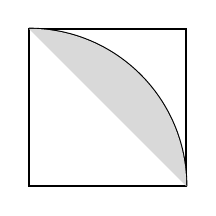
\begin{tikzpicture}[scale=2]
  \draw[thick] (0,0) rectangle (1,1);
  \draw[thick] (0,1) arc (90:0:1);
  \fill[gray!30] (0,1) arc (90:0:1) -- (1,0) -- cycle;
\end{tikzpicture}
\caption{Unit square with a quarter of a unit circle inscribed.}
\end{figure}

\subsection{Random Points}
Generate a large number of random points within the unit square. By counting the number of points that fall inside the quarter circle, we can approximate its area.

\subsection{Approximating $\pi$}
Let $N$ be the total number of random points generated and $M$ be the number of points that fall within the quarter circle. The value of $\pi$ can be approximated as:
\[
\pi \approx 4 \times \frac{M}{N}
\]

\section{Collisions of Two Squares}
Another intriguing method involves studying the collisions of two squares.

\subsection{Description}
Consider two squares of side length $l$ and $l\sqrt{2}$, placed in such a way that the smaller square is centered on one side of the larger square, and their centers are aligned.

\begin{figure}[ht]
\centering
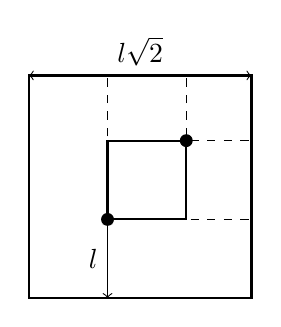
\begin{tikzpicture}
  \draw[thick] (0,0) rectangle (2.828,2.828);
  \draw[thick] (1,1) rectangle (2,2);
  \draw[<->] (0,2.828) -- (2.828,2.828) node[midway,above]{$l\sqrt{2}$};
  \draw[<->] (1,0) -- (1,1) node[midway,left]{$l$};
  \draw[dashed] (1,1) -- (1,2.828);
  \draw[dashed] (2,1) -- (2,2.828);
  \draw[dashed] (1,1) -- (2.828,1);
  \draw[dashed] (1,2) -- (2.828,2);
  \node[draw, circle, fill=black, inner sep=1.5pt] at (1, 1) {};
  \node[draw, circle, fill=black, inner sep=1.5pt] at (2, 2) {};
\end{tikzpicture}
\caption{Collisions of two squares.}
\end{figure}

\subsection{Collision Points}
When the larger square moves along a horizontal line, the smaller square moves along a vertical line, and they collide at a point. By analyzing these collision points, it is possible to calculate the value of $\pi$.

\subsection{Collisions of Two Squares - Calculations}

Let us consider the scenario of two squares as described earlier, with side lengths $l$ and $l\sqrt{2}$. We will analyze the collision points of these squares as they move along their respective paths.

Suppose the larger square starts at position $(0, 0)$ and moves horizontally along the positive $x$-axis. At time $t$, its position is given by $(x_l(t), 0)$, where $x_l(t) = vt$, and $v$ is the constant velocity of the larger square.

On the other hand, the smaller square starts at position $(0, l)$ and moves vertically along the positive $y$-axis. At time $t$, its position is given by $(0, y_s(t))$, where $y_s(t) = l - vt$, since the smaller square moves in the opposite direction to the larger square.

To find the collision point, we equate the $x$ and $y$ coordinates:
\[
x_l(t) = 0 \quad \text{and} \quad y_s(t) = 0
\]
\[
vt = 0 \quad \text{and} \quad l - vt = 0
\]

From the first equation, we get $t = 0$, which means both squares start at the origin.

Substituting $t = 0$ into the second equation, we find the $y$-coordinate of the collision point, denoted as $y_c$:
\[
y_c = l - v \times 0 = l
\]

So, the collision point is at coordinates $(0, l)$.

Now, we need to determine the time at which the collision occurs, denoted as $t_c$.

From the second equation, we have:
\[
l - vt_c = 0
\]

Solving for $t_c$, we find:
\[
t_c = \frac{l}{v}
\]

At the collision time $t_c$, the $x$-coordinate of the collision point, denoted as $x_c$, is:
\[
x_c = x_l(t_c) = v \times \frac{l}{v} = l
\]

Now, we can compute the distance from the origin to the collision point using the Pythagorean theorem:
\[
\text{Distance to collision point} = \sqrt{x_c^2 + y_c^2} = \sqrt{l^2 + l^2} = \sqrt{2l^2} = l\sqrt{2}
\]

Next, let $d$ be the distance between the centers of the two squares at the time of collision. Using the Pythagorean theorem, we can express $d$ as follows:
\[
d = \sqrt{(2l)^2 + (2l)^2} = \sqrt{8l^2} = l\sqrt{8}
\]

Since $d$ is the sum of the side lengths of the two squares, the total area covered by the two squares is given by:
\[
\text{Total Area} = (l + l\sqrt{2})^2 = l^2(1 + 2\sqrt{2})
\]

We can also calculate the area of the smaller square and the quarter circle:

\[
\text{Area of Smaller Square} = l^2
\]

\[
\text{Area of Quarter Circle} = \frac{\pi l^2}{4}
\]

Now, we can equate the total area covered by the squares to the sum of the area of the smaller square and the area of the quarter circle:

\[
l^2(1 + 2\sqrt{2}) = l^2 + \frac{\pi l^2}{4}
\]

Simplifying and solving for $\pi$, we get:

\[
\pi = \frac{4(1 + 2\sqrt{2})}{4 - \pi}
\]

Finally, we can approximate the value of $\pi$ using numerical methods like Newton-Raphson or iterative techniques.

\subsection{Approximation of $\pi$}

Using numerical methods, we can iteratively solve the equation derived in the previous section to approximate the value of $\pi$. The process involves choosing an initial guess for $\pi$, applying the iterative formula, and repeating until the desired level of accuracy is achieved. The Newton-Raphson method is one such approach that can be used to iteratively improve the approximation of $\pi$.

It is worth noting that this method provides an interesting geometric perspective on calculating $\pi$ using the collisions of two squares. Further research and exploration into this topic may lead to more advanced techniques and applications.

\section{Conclusion}
In this paper, we have explored several methods for approximating the value of $\pi$. From ancient techniques like Archimedes' method to modern probabilistic methods like Monte Carlo, each approach offers its own unique insights into the constant $\pi$. The collisions of two squares also provide a fascinating geometric approach to calculating $\pi$. These methods showcase the rich history and diversity of mathematical techniques used to understand this fundamental constant.

\end{document}